% https://conf.researchr.org/track/icsme-2025/icsme-2025-registered-reports
% Submissions to the ICSME 2025 RR track must not exceed 6 pages (plus 1 additional page of references). The page limit is strict. All submissions must be in PDF and must be submitted online by the deadline via the ICSME 2025 EasyChair link.


% 20th May last date.
\documentclass[conference,anonymous,review]{IEEEtran}

\IEEEoverridecommandlockouts


%\usepackage{csquotes}
\usepackage{cite}
\usepackage{amsmath,amsfonts,amsthm}
\usepackage{algorithm,algorithmic}
\usepackage{xspace}
\usepackage{graphicx}
\usepackage{textcomp}
\usepackage{xcolor}
\usepackage{listings}
\lstdefinestyle{Python}
{
    basicstyle=\footnotesize\ttfamily,
    numberblanklines=false,
    language=python,
    tabsize=2,
    commentstyle=\color{gray},
    keywordstyle=\bfseries\color{eclipsePurple},
    morekeywords={assert},
    stringstyle=\color{eclipseBlue},
    %procnamestyle=\bfseries\color{black},
    %procnamekeys={def},
    columns=flexible,
    identifierstyle=,
}
\definecolor{eclipseBlue}{RGB}{42,0.0,255}
\definecolor{eclipseGreen}{RGB}{63,127,95}
\definecolor{eclipsePurple}{RGB}{127,0,85}
\usepackage{multirow}
\usepackage{pifont}% http://ctan.org/pkg/pifont
\usepackage{hyperref}
\newcommand{\mytitle}{Assessing Reliability of Statistical Maximum Coverage Estimators in Fuzzing}
\hypersetup{pdftitle={\mytitle},
colorlinks=true,linkcolor=blue,citecolor=blue,filecolor=blue,urlcolor=blue
}
\usepackage{tikz}
\usepackage{pgfplots}
\usepackage{balance}
\pgfplotsset{compat=1.9}
\usetikzlibrary{fit}
\usetikzlibrary{positioning}
\usetikzlibrary{datavisualization,datavisualization.formats.functions}
\usetikzlibrary{shapes, calc, decorations, automata}
\usetikzlibrary{shapes.geometric, arrows}
\usetikzlibrary{decorations.markings}
\usetikzlibrary{arrows.meta}
\usetikzlibrary{chains,shadows.blur}
\usetikzlibrary{math}
\usepgfplotslibrary{fillbetween}
\tikzstyle{startstop} = [rectangle, rounded corners, minimum width=3cm, minimum height=1cm,text centered, draw=black, fill=red!30]
\tikzstyle{process} = [rectangle, rounded corners, minimum width=3cm, minimum height=1cm, text centered, draw=black, fill=orange!30, inner sep=5pt,minimum size=10pt]
\tikzstyle{decision} = [diamond, minimum width=3cm, minimum height=1cm, text centered, draw=black, fill=green!30]
\tikzstyle{arrow} = [thick,->,>=stealth]
\usepackage{cleveref}
\usepackage{subcaption}

%\usepackage{subfig,paralist}
\usepackage{pifont}
\usepackage{enumitem}
\usepackage{url}
\usepackage{booktabs}
\usepackage{tabularx}
\usepackage{multirow,array}
\usepackage{threeparttable}
%\usepackage{balance}
%\usepackage[group-separator={,}]{siunitx}
%\usepackage[capitalise]{cleveref}
\usepackage{bm}
\usepackage{syntax}
%% Identifiers
\def\|#1|{\textit{#1}}
\def\<#1>{\texttt{#1}}
\def\[[#1\]]{\texttt{#1}}

\def\term#1{\texttt{'\textbf{#1}'}}
\def\nonterm#1{\textlangle\textnormal{\emph{#1}}\textrangle}
\def\regex#1{\texttt{{\color{blue}/}#1{\color{blue}/}}}
\def\expandsto{\(\rightarrow{}\)}
\usepackage{bbding}
\DeclareUnicodeCharacter{1F3B2}{\dice}

\usepackage{wrapfig}
\usepackage{tikz}
\usetikzlibrary{shapes, calc, decorations, automata}
\usetikzlibrary{shapes.geometric, arrows}
\usetikzlibrary{decorations.markings}
\usetikzlibrary{arrows.meta}
\usetikzlibrary{chains,shadows.blur}


\newcounter{todocounter}
\newcommand{\todo}[1]{\marginpar{$|$}\textcolor{red}{\stepcounter{todocounter}\footnote[\thetodocounter]{\textcolor{red}{\textbf{TODO }}\textit{#1}}}}
\newcommand{\done}[1]{\marginpar{$*$}\textcolor{green}{\stepcounter{todocounter}\footnote[\thetodocounter]{\textcolor{black}{\textbf{DONE }}\textit{#1}}}}

\newcommand{\recheck}[1]{\textcolor{red}{#1}}
\newcommand{\revise}[1]{\textcolor{black}{#1}}

\renewcommand{\done}[1]{} % comment to see responses.

% Hide TODOs for final version if needed
% \IfFileExists{SUBMIT}{ % Requires creating a file named SUBMIT
% \renewcommand{\todo}[1]{}
% \renewcommand{\done}[1]{}
% }{}
% \usepackage{colortbl} % Already loaded




\usepackage{tikz}
\newcommand*\circled[1]{\tikz[baseline=(char.base)]{
            \node[shape=circle,draw,inner sep=2pt] (char) {#1};}}
\urlstyle{tt}

\def\BibTeX{{\rm B\kern-.05em{\sc i\kern-.025em b}\kern-.08em
    T\kern-.1667em\lower.7ex\hbox{E}\kern-.125emX}}

\newtheorem{theorem}{Theorem}
\newtheorem*{theorem*}{Theorem}
\newtheorem{lemma}{Lemma}
%\renewcommand\qedsymbol{$\blacksquare$}
\newcommand*\diff{\mathop{}\!\mathrm{d}}

\usepackage{tcolorbox}% http://ctan.org/pkg/tcolorbox
\definecolor{mycolor}{rgb}{0.122, 0.435, 0.698}% Rule colour
\definecolor{gray1}{gray}{0.3}

\definecolor{codegreen}{rgb}{0,0.6,0}
\definecolor{codegray}{rgb}{0.5,0.5,0.5}
\definecolor{codepurple}{rgb}{0.58,0,0.82}
\definecolor{backcolour}{rgb}{0.95,0.95,0.92}
\lstdefinestyle{mystyle}{
    %backgroundcolor=\color{backcolour},
    commentstyle=\color{codegreen},
    keywordstyle=\color{magenta},
    numberstyle=\tiny\color{codegray},
    stringstyle=\color{codepurple},
    basicstyle=\tiny\ttfamily,
    breakatwhitespace=false,
    breaklines=true,
    captionpos=b,
    keepspaces=true,
    numbers=left,
    numbersep=5pt,
    showspaces=false,
    showstringspaces=false,
    showtabs=false,
    tabsize=2,
    columns=fixed
}
\lstset{style=mystyle}

\newcommand{\result}[1]{%
\begin{tcolorbox}[colframe=black,boxrule=0.5pt,arc=4pt,
      left=6pt,right=6pt,top=6pt,bottom=6pt,boxsep=0pt,width=\columnwidth]%
      {\emph{#1}}
\end{tcolorbox}%
}

\definecolor{darkgreen}{rgb}{0.0, 0.5, 0.0}
\definecolor{darkred}{rgb}{0.82, 0.1, 0.26}
\newcommand{\cmark}{\textcolor{darkgreen}{\ding{51}}}%
\newcommand{\xmark}{\textcolor{darkred}{\ding{55}}\ }%

\def\sectionautorefname{Section}
\def\subsectionautorefname{Section}
\def\subsubsectionautorefname{Section}%%

\begin{document}

\title{\mytitle}

% \author{
% \IEEEauthorblockN{Danushka Liyanage}
% \IEEEauthorblockA{\textit{School of Computer Science} \\
% \textit{University of Sydney}\\
% Sydney, Australia \\
% danushka.liyanage@sydney.edu.au}
% \and 
% \IEEEauthorblockN{Rahul Gopinath}
% \IEEEauthorblockA{\textit{School of Computer Science} \\
% \textit{University of Sydney}\\
% Sydney, Australia \\
% rahul.gopinath@sydney.edu.au}
% }

\maketitle

\thispagestyle{plain}
\pagestyle{plain} 


\begin{abstract}
Fuzzers are often guided by coverage, making the estimation of maximum 
achievable coverage a key concern in fuzzing.
However, achieving 100\% coverage is infeasible for most real-world
software systems, regardless of effort.
While static reachability analysis can provide an upper bound,
it is often highly inaccurate.
Recently, statistical estimation methods based on species richness
estimators from biostatistics have been proposed as a potential solution.
Yet, the lack of reliable benchmarks with labeled ground truth has
limited rigorous evaluation of their accuracy.

To address this challenge, we propose an evaluation framework that
synthetically generates large programs with complex control flows,
ensuring well-defined reachability and providing ground truth for evaluation.
Additionally, we propose a novel reliability check for these estimators
on real-world benchmarks without labeled ground truth—by varying the size
of sampling units, which, in theory, should not affect the estimate.

Our work aims to identify the most reliable methods for estimating
maximum achievable coverage in practical fuzzing campaigns.
\end{abstract}


\section{Introduction}

Fuzzing is an automated testing technique that leverages guidance provided
by coverage~\cite{boehme2016coverage}.
The budget allocated to fuzzing, and hence, the stopping criteria
of fuzzing is strongly determined by the maximum possible coverage that can
be obtained~\cite{fell2017review}.
%
However, achieving 100\% coverage in complex real-world programs is practically impossible~\cite{horgan1994achieving}. 
As the input domain and execution space grow, exhaustive testing becomes infeasible~\cite{knight1996exhaustive}.

Yet, quantifying the maximum reachable coverage (also called \emph{maximum reachability}) remains a challenge, raising a fundamental question:
\emph{How close is a fuzzing campaign to its maximum reachable coverage?}

Recent researches have proposed \emph{species richness estimators} from
biostatistics~\cite{chao2016species} as a principled approach to estimate
the reachable coverage of a fuzzing campaign~\cite{boehme2018stads}.
These estimators model fuzzing as a statistical sampling process where
each test input exercises one or more program behaviors---such as reaching
a program element---which can then be used to estimate the total number of such behaviors~\cite{boehme2018stads}.

However, evaluating the accuracy and reliability
of these estimators is difficult. The main issue is that, to evaluate such
estimators, we need a benchmark of several large complex programs where
maximum reachability is known \cite{liyanage2021security}. Unfortunately, establishing the maximum
reachability is impossible except for trivial programs. Hence, researchers have resorted to using small programs, fuzzed to saturation as an alternative~\cite{liyanage2023reachable}.
This approach is not ideal as the performance of an estimator in small  
programs may not be representative of the performance of an estimator in complex
real-world programs (such as the benchmarks in Fuzzbench \cite{metzman2021fuzzbench}).

We propose an alternative approach to overcome this difficulty. We note that
in programs such as parsers (which are one of the major subjects for fuzzing)
the control-flow of a program along with its data-flow determines the
complexity of the program, and hence, determines the difficulty
experienced in reaching the program elements. The control-flow of any
structured program can be represented as a context-free
grammar~(see for e.g., \Cref{fig:cfg}).

We note that it is possible to generate arbitrary
context-free grammars. Furthermore, one can also fine-tune the complexity
of such grammars generated based on several dimensions such as the size
of the grammar, the number of direct and indirect recursions allowed, the
number of linear-recursive rules etc.
Finally, converting a context-free grammar to recursive descent
parsers is well known, and produces parsers which have similarly complex
control-flows.

Our proposal is then to leverage such arbitrarily generated complex
context-free grammars into parsers, and use such parsers as benchmarks for
estimating the reliability of reachability estimators. We propose to compare
the difficulty of fuzzers when faced with real-world parsers to these
generated parsers to ensure that the generated benchmarks are similar to
real-world programs in complexity. If they prove equivalent in complexity,
such generated, and ever-renewable benchmarks may not only be suitable for
evaluating the reliability of estimators, but also for other evaluation
tasks that require complex programs such as evaluating fuzzers,
fault localization techniques, program repair techniques, and so on.

\begin{figure*}
\begin{subfigure}[h]{0.3\textwidth}
\centering
%
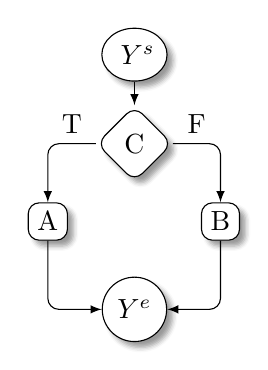
\begin{tikzpicture}[auto,
  node distance = 3mm,
  start chain = going below,
  start/.style = {ellipse,draw,text width= 1em,rounded corners,blur shadow,fill=white,
        on chain,align=center},
  box/.style = {draw,rounded corners,blur shadow,fill=white,
        on chain,align=center},
  cond/.style = {diamond,draw,rounded corners,blur shadow,fill=white,
        on chain,align=center},
  stop/.style = {circle,minimum width=20pt,draw,blur shadow,fill=white,
        on chain,align=center}
]
 \node[start] (b1)    {$Y^s$};
 \node[cond] (b2)    {C};
 \node[box, below left=0.5cm and 0.6cm of b2] (b21) {A};
 \node[box, below right=0.5cm and 0.6cm of b2] (b22) {B};
 \node[stop,below=12mm of b2] (b3)    {$Y^e$};
 \begin{scope}[rounded corners,-latex]
 \path
 (b1) edge (b2);
 \draw[-latex] (b2) -| node[pos=0.25,above] {T} (b21);
 \draw[-latex] (b2) -| node[pos=0.25,above] {F} (b22);
  \draw[-latex] (b21) |- (b3);
  \draw[-latex] (b22) |- (b3);
\end{scope}
\end{tikzpicture}
\caption{Condition}
\label{tikz:condition}
\end{subfigure}
\begin{subfigure}[h]{0.3\textwidth}
\centering
% \vspace{2.8cm}
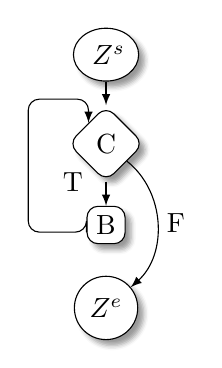
\begin{tikzpicture}[auto,
  node distance = 3mm,
  start chain = going below,
  start/.style = {ellipse,draw,text width= 1em,rounded corners,blur shadow,fill=white,
  on chain,align=center},
  box/.style = {draw,rounded corners,blur shadow,fill=white,
  on chain,align=center},
  cond/.style = {diamond,aspect=1,draw,rounded corners,blur shadow,fill=white,
  on chain,align=center},
  stop/.style = {circle,minimum width=20pt,draw,blur shadow,fill=white,
  on chain,align=center}]
 \node[start] (b1)    {$Z^s$};      
 \node[cond] (b2)    {C};      
 \node[box] (b3)    {B};  
 %\node[stop] (b4)    {e};
 \node[stop,below=4mm of b3] (b4)    {$Z^e$};
 \begin{scope}[rounded corners,-latex]
  \path (b2.-40) edge[bend left=50] node[midway,right] {F} (b4.40)
  (b1) edge node [midway,below, xshift=-12pt,yshift=-25pt] {T}(b2)
  (b2) edge (b3);
  \draw (b3.200) -- ++(0,0) -| ([xshift=-5mm]b2.west) |-
  ([yshift=3mm]b2.130) -- (b2.130);
 \end{scope}
\end{tikzpicture}
\caption{Iteration}
\label{tikz:iteration}
\end{subfigure}
\begin{subfigure}[h]{0.3\textwidth}
\centering
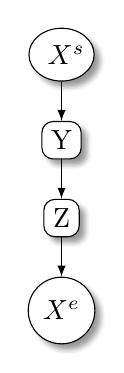
\begin{tikzpicture}[auto,
  node distance = 3mm,
  start chain = going below,
  start/.style = {ellipse,draw,text width= 1em,rounded corners,blur shadow,fill=white,
        on chain,align=center},
  box/.style = {draw,rounded corners,blur shadow,fill=white,
        on chain,align=center},
  stop/.style = {circle,minimum width=20pt,draw,blur shadow,fill=white,
        on chain,align=center}]
 \node[start] (b1)    {$X^{s}$};
 \node[box,below=5mm of b1] (b2)    {Y};
 \node[box,below=5mm of b2] (b3)    {Z};
 \node[stop,below=5mm of b3] (b4)    {$X^{e}$};
 \begin{scope}[rounded corners,-latex]
  \path
  (b1) edge (b2)
  (b2) edge (b3)
  (b3) edge (b4);
 \end{scope}
\end{tikzpicture}
\caption{Sequence}
\label{tikz:sequence}
\end{subfigure}
\vspace{10pt}

\begin{subfigure}[h]{0.3\textwidth}
\begin{grammar}\centering
    <Y> $\rightarrow$ <C> \term{T} <A> | <C> \term{F} <B>
\end{grammar}
\end{subfigure}
\begin{subfigure}[h]{0.3\textwidth}
\begin{grammar}\centering
  <Z> $\rightarrow$ <C> \term{T} <B> <Z> | <C> \term{F}
\end{grammar}
\end{subfigure}
\begin{subfigure}[h]{0.3\textwidth}
\begin{grammar}\centering
  <X> $\rightarrow$ <Y> <Z>
\end{grammar}
\end{subfigure}
%
\caption{The basic control-flow structures}
\label{fig:cfg}
\end{figure*}

While synthetic benchmarks are a useful alternative, is it possible to use
real-world programs even if ground-truth (the maximum reachability) is not
known? A recent research on evaluating the reliability of biostatistics based
estimators for mutation analysis~\cite{Kuznetsov2024empirical} provides a
solution. The researchers point out that the \emph{sampling units} used in
species richness estimators should not have a significant effect on the final
estimate. In previous research on coverage estimation~\cite{liyanage2023reachable},
the sampling-unit used is the time interval. That is, the incidence data of
each 15-minutes bin was used as the sampling unit. Since the 15-minute interval
is arbitrary, it stands to reason that changing the timing granularity should
not impact the final estimate. Hence, we propose to evaluate the reliability of
maximum coverage estimators under varying granularity of sampling interval,
for the same fuzzing campaign duration.

\noindent{}\textbf{Contributions:}

\begin{itemize}
  \item \textbf{Synthetic benchmarks for evaluation:} We propose a novel
framework to generate synthetic program benchmarks that emulates real-world
programs, and use this to evaluate maximum reachability estimators.

  \item \textbf{Sampling-unit based evaluation of reliability:} We will evaluate
    the reliability of maximum reachability estimators on 32 real-world programs
    by comparing the estimates under sampling units of diverse granularity.

\end{itemize}

The remainder of this paper is organized as follows. Section~\ref{sec:preliminaries} introduces the statistical reachability estimation and evaluation in fuzzing. Section~\ref{sec:method} presents our methodology for assessing the accuracy and reliability of statistical estimators of maximum reachability. Section~\ref{sec:setup} details the experimental setup used to evaluate our approach. Then, Section~\ref{sec:related} and Section~\ref{sec:threats} discuss the associated related work and threats to validity. Finally, Section~\ref{sec:conclusion} concludes the paper and outlines directions for future research.

\section{Preliminaries} \label{sec:preliminaries}
In this section, we first explain the theoretical underpinnings of the reachability estimation models. Next, we introduce the context-free grammar, and explain
the control-flow graphs.
\subsection{Computing Maximum Reachability}
\label{sec:reachability}
To evaluate fuzzer effectiveness, we need the maximum reachability in a given program, which is often unavailable, and hence need to be approximated. We next discuss the major approaches for approximation.

\noindent\textbf{Non-statistical approaches:} 
\begin{enumerate}
    \item \emph{Plateaued Coverage~\cite{boehme2018stads}:} Previous research treated the observed coverage at the end of a fuzzing campaign when coverage plateaued as the ground truth. However, given the exponential difficulty of finding new behaviors~\cite{boehme2021residual}, this approach is unsatisfactory.
    \item \emph{Small-scale Programs~\cite{liyanage2023reachable}:} For programs with limited behavioral diversity, fuzzers often reach coverage saturation quickly, which can be a source of ground truth. However, they lack the complexity of real-world programs, and are a poor substitute for good benchmarks.
\end{enumerate}
    
\noindent\textbf{Statistical approaches:} 
\begin{enumerate}
    \item \emph{Bootstrapping~\cite{liyanage2023reachable}:} 
    Once coverage stabilizes, bootstrapping/resampling from campaign data can statistically approximate ground truth. However, it relies on assumptions such as independence of inputs, and relative homogeneity of behavioral complexity in unreached regions. 
    \item\emph{Species richness estimators:} We evaluate all species-richness estimators used by Liyanage et al.~\cite{liyanage2023reachable}. Additionally, inspired by recent studies on estimator performance for estimating maximum mutation score~\cite{Kuznetsov2024empirical}, we incorporate further estimators---including \emph{bootstrap}~\cite{smith1984nonparametric}, \emph{Zelterman}~\cite{bohning2010some}, and others\todo{Fill in all}. While promising, species-richness estimators have similar assumptions as that of bootstrapping, which may not be reasonable in real-world programs.
\end{enumerate}
% Prior empirical research on estimating maximum reachable coverage in fuzzing
% campaigns—under the Bernoulli product model—has shown that statistical
% estimators systematically underestimate true reachability until near
% saturation, a phenomenon termed \emph{false peaks}~\cite{liyanage2023reachable}.
% This negative bias is largely inevitable in early stages due to the
% insufficiency of fuzzing data and the heterogeneous species diversity,
% which limits accurate approximation of the species distribution.
% 
% Prior research~\cite{liyanage2023reachable} empirically investigated this
% phenomenon, and suggests that estimators become reliable when the
% count of doubletons equals or exheeds singletons.
We next discuss the statistical approaches in detail.
\subsubsection{Probabilistic Model for Fuzzing}
The STADS\footnote{STADS—Software Testing As Discovery of Species} framework~\cite{boehme2018stads,boehme2021residual,nguyen2022bedivfuzz,boehme2020boosting} formalizes
fuzzing as a statistical sampling process $\mathcal{F}$. Each test input is drawn with replacement from the program's input space $\pmb{\mathcal{D}}$. Assuming a sequence of $N$ independent and identically distributed (i.i.d.) random variables are drawn, we formally define the fuzzing campaign $\mathcal{F}$ as:

\begin{equation*}
    \mathcal{F}=\{X_n \mid X_n \in \pmb{\mathcal{D}}\}_{n=1}^N
\end{equation*}

The input space $\pmb{\mathcal{D}}$ consists of $S$ (potentially overlapping) subdomains $\{\mathcal{D}_i\}_{i=1}^S$, each representing a distinct \emph{coverage element}. An input $X_n \in \mathcal{F}$ is said to discover a \emph{new} coverage element $\mathcal{D}_i$ if $X_n \in \mathcal{D}_i$ and no earlier input $X_m \in \mathcal{F}$ for $m < n$ has been drawn from $\mathcal{D}_i$—that is, $\mathcal{D}_i$ is being encountered for the first time.

\begin{figure*}[ht] %{r}{7cm} %[12]
  \centering
\begin{subfigure}[h]{0.45\textwidth} %22 min
  \centering
\lstset{numbers=left,xleftmargin=2em, numberstyle=\color{lightgray}
} %frame=single,framexleftmargin=1.5em}
\begin{lstlisting}[style=Python, escapechar=|,numbersep=2pt]
def bsearch(x, v, n):
  low, high = 0, n-1
  while low <= high:
    mid=(low+high)/2
    if x < v[mid]:
      high=mid-1
    else:
      if x > v[mid]:
        low=mid+1
      else:
        return mid
  return None
\end{lstlisting}
\caption{\<bsearch> program}
\label{fig:bsearch1}
\end{subfigure}
\begin{subfigure}[h]{0.45\textwidth}   %28 min
  \centering
\begin{grammar}%\centering
  <bsearch> $\rightarrow$ \term{l.2} <while.3> \term{l.12}

  <while.3> $\rightarrow$ \term{l.3}
   \alt \term{l.3} \term{l.4} \term{l.5} <if.5> <while.3>

  <if.5>  $\rightarrow$  \term{T} \term{l.6}
   \alt \term{F} \term{l.8} <if.8>

  <if.8> $\rightarrow$ \term{T} \term{l.9}
   \alt \term{F} \term{l.11}
\end{grammar}
\caption{\<bsearch> control-flow equivalent grammar}
\label{fig:bsearch3}
\end{subfigure}
\caption{Equivalent context-free grammar for \<bsearch> program control-flow}
\label{fig:bsearch}
\end{figure*}

\subsubsection{Bernoulli Product Model}
Since each input in $\mathcal{F}$ may belong to one or more coverage elements, the STADS model represents coverage using \emph{sampling-unit-based incidence data}~\cite{colwell2012models,chao2017thirty}, where a sampling unit aggregates all inputs generated within a fixed time interval. The underlying probabilistic model for this representation is the \emph{Bernoulli product model}. Grouping inputs into sampling units is essential to reduce the overhead of tracking fine-grained coverage information for each individual input during fuzzing.

For each sampling unit, the collected data indicates whether a coverage element
has been reached. Let $\pi_i$ denote the probability that a sampling unit covers
element $\mathcal{D}_i$, assuming $\pi_i$ remains constant across all randomly
selected sampling units.
In general, the sum of all $\pi_i$ values does \emph{not} equal unity.

During a fuzzing campaign, suppose we record $t$ sampling units. The incidence data forms an element$\times$sampling-unit incidence matrix ${W_{ij};i=1,2,\dots,S,j=1,2,\dots,t}$ with $S$ rows and $t$ columns, where $W_{ij} = 1$ if element $i$ is covered in sampling unit $j$, and $W_{ij} = 0$ otherwise.

The incidence frequency $Y_i$ represents the number of sampling units in which element $\mathcal{D}_i$ is covered; i.e., $Y_i=\sum_{j=1}^{t}W_{ij}$. A coverage element $\mathcal{D}_i$ that has not been covered by any sampling unit will have an incidence frequency of zero; i.e., $Y_i=0$.

Given the set of detection probabilities $(\pi_1,\pi_2,\dots,\pi_S)$, we assume each element $W_{ij}$ in the incidence matrix follows a Bernoulli distribution with probability $\pi_i$. The probability distribution for the incidence matrix is:

\begin{equation}
    \begin{split}
        P(W_{ij}=w_{ij};i=1,2,\dots,S,j=1,2,\dots,t) \\
        = \prod_{j=1}^{t}\prod_{i=1}^{S}\pi_i^{w_{ij}}(1-\pi_i)^{1-w_{ij}} \\
        = \prod_{i=1}^{S}\pi_i^{y_i}(1-\pi_i)^{t-y_i}.
    \end{split}
\end{equation}

The marginal distribution for the incidence-based frequency $Y_i$ for the $i$-th coverage element follows a binomial distribution characterized by $t$ and the detection probability $\pi_i$:

\begin{equation}
    P(Y_i=y_i) = \binom{t}{y_i}\pi_i^{y_i}(1-\pi_i)^{t-y_i}, \qquad i=1,2,\dots,S.
\end{equation}

Denote the incidence frequency counts by $(f_0, f_1, \dots, f_t)$, where $f_k$ is the number of elements covered in exactly $k$ sampling units in the data, $k=0,1,\dots,t$. Here, $f_1$ represents the number of \emph{singleton} elements (those that are covered in only one sampling unit), and $f_2$ represents the number of \emph{doubleton} elements (those that are covered in exactly two sampling units). The unobservable zero frequency count $f_0$ denotes the number of coverage elements that are not covered by any of the $t$ sampling units. Then, the number of covered elements in the current campaign is $S(t)=\sum_{i>0}f_i$, and $S(t)+f_0=S$.

\section{Methodology} \label{sec:method}
We next describe our methodology for generation of synthetic benchmarks.
Since the maximum reachability in these programs are controlled, we will use
these programs to evaluate the reliability of estimators.
\subsection{Synthetic Benchmarks With Known Reachability}
We generate large programs with complex control flow by leveraging the
structural isomorphism between control-flow graphs and context-free grammars.

\noindent\textbf{Primer on Context-Free Grammars.}
A context-free grammar (also called a \emph{grammar})
is a formal system for defining a language. The following is a simple grammar:
\begin{grammar}\centering
<E> $\rightarrow$ <T> \term{+} <E> $\mid$ <T>

<T> $\rightarrow$ \term{0} $\mid$ \term{1} \phantom{a} \phantom{a} \phantom{a} \phantom{a}
\end{grammar}

The alphabets of the language are called \emph{terminal symbols}. In the above \term{0} is
a terminal symbol.
The grammar also contains \emph{nonterminal symbols} which are named
constructs that can be expanded into other terminal or nonterminal
symbols (e.g., \nonterm{E} in the above).

How the nonterminal symbols are expanded into other symbols is defined
by a set of \emph{production rules}, which together form the definition of that
nonterminal symbol. In the above example, the definition of the nonterminal \nonterm{E} is given
by
\mbox{\nonterm{E} \expandsto \nonterm{T} \term{+} \nonterm{E} $\mid$ \nonterm{T}} which
contains two rules for expanding \nonterm{E}.

\noindent\textbf{From Control-Flow to Grammar.}
A control-flow graph represents the possible execution paths of a program and is
typically modeled as a directed graph.
\Cref{fig:cfg} illustrates example control-flow graphs for three procedures:
\<Y>, \<Z>, and \<X>.
Each graph consists of a set of nodes $N$, where each node $N_i$ represents a
program statement\footnote{Traditionally, a node corresponds to a basic block,
but for the purposes of this work, we treat each node as a single statement without loss of generality.}.
Edges $E_{i,j}$ define possible control transfers, including:
\begin{itemize}
    \item \textbf{Sequential}, representing sequential execution;
    \item \textbf{Conditional}, for branching (e.g., \<if-then-else>);
    \item \textbf{Loop}, modeling iteration (e.g., \<while> loops);
    \item \textbf{Call}, connecting to other procedures.
\end{itemize}

These control-flow structures map naturally to production rules in a
context-free grammar. Specifically:
\begin{itemize}
    \item Conditionals such as \<if C: A else: B> map to
      \mbox{\nonterm{IF} \expandsto \nonterm{C} \term{T} \nonterm{A}  $|$ \nonterm{C} \term{F} \nonterm{B}};
    \item Loops such as \<while C: B> map to
      \mbox{\nonterm{L} \expandsto \nonterm{C} \nonterm{B} \nonterm{L} $|$ \nonterm{C}};
    \item Procedure definitions translate to corresponding nonterminals.
\end{itemize}
\Cref{fig:bsearch} shows the equivalent context-free grammar from a given
program.

This means that the space of all possible context-free grammars covers the space
of all structured program control-flows.

\noindent\textbf{From Grammar to Executable Programs.}
Given any non-left-recursive context-free
grammar, we can generate a recursive-descent parser using these rules:
\begin{itemize}
  \item Each nonterminal becomes a function. For example, \nonterm{E} is translated to \<def parse\_E>.
  \item Each production rule is implemented in that function.
  \item Lookahead tokens guide which rule to apply.
  \item Linear recursion can be replaced with a \<while> loop.
\end{itemize}

Following in this fashion, we get a parser that directly corresponds to the context-free
grammar. For example, given the grammar
\begin{grammar}\centering
  <E> $\rightarrow$ <D> <Es>\phantom{a}\phantom{a}\phantom{a}\phantom{a}\phantom{a}\phantom{a}\phantom{a}\phantom{a}

<Es> $\rightarrow$ \term{+} <D> <Es> $\mid$ $\epsilon$
\end{grammar}
we can translate this to:
\begin{lstlisting}[style=Python, escapechar=|,numbersep=2pt]
def parse_E():
  parse_D()

  while lookahead() == '+':
    consume('+')
    parse_D()
  return node

def parse_D():
  token = lookahead()
  if token and isdigit(token):
    consume(token)
  else:
    raise Error()
\end{lstlisting}
which has similar control-flow as a program from which such a grammar may have
been obtained.


% Each nonterminal becomes a parser function, and each production rule is
% implemented as control-flow branches in that function. For example, given the grammar:
% 
% \begin{grammar}\centering
%   <E> $\rightarrow$ <D> <Es>\phantom{a}\phantom{a}\phantom{a}\phantom{a}\phantom{a}\phantom{a}\phantom{a}\phantom{a}\phantom{a}
% 
% <Es> $\rightarrow$ \term{+} <D> <Es> $\mid$ $\epsilon$
% \end{grammar}
% 
% we generate the following parser:
% 
% \begin{lstlisting}[style=Python, escapechar=|,numbersep=2pt]
% def parse_E():
%   parse_D()
%   while lookahead() == '+':
%     consume('+')
%     parse_D()
%   return
% 
% def parse_D():
%   token = lookahead()
%   if token and isdigit(token):
%     consume(token)
%   else:
%     raise Error()
% \end{lstlisting}
% 
% This parser mirrors the control-flow structure of the original grammar.

\noindent\textbf{Controlling the program complexity.}
While generating context-free grammars, we have several mechanisms to
precisely control the complexity. These include:

\begin{itemize}
    \item The number of nonterminals (corresponding to the number of procedures),
    \item The number and length of production rules (corresponding to branching complexity),
    \item The depth and type of recursion (direct, indirect, or linear recursion),
    \item The inclusion of unreachable nonterminals or dead code to simulate partially unreachable programs.
% \item The number and kind of alphabets in the language. A larger set of alphabets 
% \item The VC dimension of the language.
\end{itemize}

These parameters allow us to generate large structured parser programs with
complex control-flows. We can additionally increase the difficulty level by
adding extra constraints to the generated parser such
as context-sensitivity.

To prevent trivial estimation (e.g., estimators that always return 100\%),
we introduce unreachable elements by including nonterminals that are not
reachable from the start symbol.
We may also wrap parser call-sites with guards or inject dead branches.

\subsection{Assessing Reliability of \texorpdfstring{$\hat{S}$}{S-hat} Estimators Without Ground truth}
To overcome any limitation that may exist due to the synthetic nature of our
previously proposed benchmark, we propose a second criterion that can be applied
to real-world benchmarks without relying on the availability of ground truth.

Our approach is inspired by the previous research on equivalent mutant
estimation~\cite{Kuznetsov2024empirical}, which suggests that varying
sample-units can be leveraged to evaluate the reliability of estimators.
The idea is that, while incidence-based statistical estimators of
fuzzing effectiveness may be sensitive to the sampling unit size ($r$),
a reliable estimator should produce overlapping point estimates for $S$—with
varying variance but consistent expectation when evaluated over equal-length
campaigns.

We propose to evaluate whether estimators of maximum reachability $S$ yield
consistent point estimates with overlapping confidence intervals, while allowing
for differences in estimation accuracy (i.e., variability) across fuzzing
campaigns with different sampling unit definitions $r$.

\section{Experimental Setup}
\label{sec:setup}
We describe the details our proposed experiment here.
\subsection{Research Questions}
How well do the current techniques for estimating the maximum reachability
of statements in a program perform? What are their limitations? Can the
point estimators be trusted? and are the confidence intervals obtained accurate?
The following research question will be investigating each of these points.

\noindent\textbf{RQ1:} How accurate are the estimators of maximum reachability
in terms of the point estimate as well as the confidence intervals?

The second question that we want to be answered is regarding the reliability
of the sampling units used in species richness based statistical estimators for
maximum reachability. We note that there are several methods for formulating
the problem of maximum reachability as a species richness estimate. For example,
if one is using traditional test cases, the sampling unit can be the test
classes and test methods as Kuznetsov et al.~\cite{Kuznetsov2024empirical}
demonstrates. On the other hand, in the case of fuzzing, where there is no
simple mechanism to identify non-overlapping sampling units, one can use the
incidence data under various time intervals as
Liyanage et al.~\cite{liyanage2023reachable} demonstrates. In both these cases, the
sampling units can be varied. In particular, Liyanage et al. chose 15~minutes
as the time interval for sampling unit. However, it can be asked if a time
interval of 5 minutes or even 60 minutes would have similar estimates.
The following research question will investigate this question.

\noindent\textbf{RQ2:} To what extent are the estimates of maximum reachability
$S$ sensitive to changes in the sampling unit size $r$?

\subsection{Fuzzers and Subject Programs}

For our experiments, we use AFL++ \cite{fioraldi2020AFL++}, a widely recognized state-of-the-art greybox fuzzer known for its performance and extensive adoption in recent research, particularly in reachability estimation studies. Using the same fuzzer as prior work enables direct and fair comparisons when evaluating estimator performance (RQ2).

As detailed in Section~\ref{sec:method}, we select a diverse set of large C parsers with known ground truth as our fuzzing benchmarks. We ensure that these targets are compatible with AFL++ and suitable for large-scale fuzzing experiments. \todo{Indicate the specific number of subjects/parsers etc.}

\subsection{Evaluation Metrics}
To assess the performance of statistical estimators of maximum reachability, we adopt
the following metrics, covering both accuracy and reliability.
\begin{enumerate}
\item \textbf{Point estimate bias.} We define the bias as the difference between the estimator's
point estimate $\hat{S}$ and the known ground truth $S$ available from the synthetic benchmark.
Formally,
\begin{equation}
\text{Bias} = \hat{S} - S
\end{equation}
A smaller absolute bias indicates better estimate accuracy. We will report the mean bias over
multiple runs.
\item \textbf{Confidence interval coverage.} When estimators provide confidence intervals, we will evaluate their coverage by checking whether the true $S$ lies within the specified interval. We will report the proportion of CIs containing the true $S$.
\item \textbf{Variance across multiple runs.} Variance quantifies the stability of the
estimator across multiple fuzzing campaigns. For each estimator, we will report the variance
of $\hat{S}$ over repeated trials. Low variance indicates greater stability and robustness of the estimation.
\item\textbf{Sampling unit sensitivity.} We will consider an estimator reliable if its
point estimates across different time intervals have overlapping confidence intervals, and
no significant shifts in mean estimates. We will use Welch's t-test to test whether the 
observations are significantly different. A reliable estimator should result in no significant
differences.
\end{enumerate}


\section{Related Work}
\label{sec:related}

Reachable program behaviors (e.g. code coverage and discovered bugs) determine the \emph{effectiveness} of a software testing process. For non-trivial programs, exhaustively exercising all possible behaviors is infeasible. Consequently, testing is often viewed as a means to demonstrate the presence of bugs, but not their absence~\cite{dijkstra2022reliability}. Despite this limitation, substantial effort has been directed toward increasing maximum reachability to enhance software security and reliability. Nevertheless, determining reachability remains a fundamental challenge in software testing. In fact, an efficient and precise determination of reachable code would effectively resolve the software verification problem~\cite{liyanage2023reachable}. 

Efforts to approximate reachability quantitatively have gained traction in the security domain, despite inherent difficulties. Empirical studies indicate that establishing the reachability of certain code regions is particularly challenging in large, complex code bases, using both static and dynamic analysis techniques~\cite{latoza2010developers}. Static analysis methods, such as symbolic execution, often suffer from over- or under-approximation when estimating reachable coverage~\cite{liyanage2023reachable,aniche2015why}. For instance, Nikoli\'{c} and Spoto~\cite{nikolic2013reachability} proposed approximating the reachability of program variables as a new abstract domain for static analysis. While their approach yields over-approximations, authors argue that it can be conservatively applied to identify unreachable code. Similarly, Mikol\'{a}\v{s} et al.~\cite{janota2007reachability} leveraged annotated code to define unreachability conditions and proposed an efficient algorithm for detecting unreachable code.

To assess reachability or unreachability in dynamic analysis, both constraint-solving techniques such as SMT\footnote{SMT—Satisfiability Modulo Theory} and data-driven estimation methods have been explored. Naus et al.~\cite{naus2023low} proposed a technique for automatically generating preconditions to trigger specific post-conditions (e.g., bugs) using low-level code analysis. Similarly, Liew et al.~\cite{liew2019just} demonstrated how to encode SMT formulas within coverage-guided fuzzers to discover inputs that reach targeted program locations. In contrast, statistical approaches directly attempt to estimate the test effectiveness (aka maximum reachability) through observed behaviors. The pioneering STADS framework~\cite{boehme2018stads} introduced a suite of bio-statistical estimators by modeling fuzzing as a statistical sampling process. A recent evaluation of these estimators highlighted key challenges associated with reachability estimation~\cite{liyanage2023reachable}. When applied to estimate the number of killable mutants in mutation analysis, Kuznetsov et al.~\cite{Kuznetsov2024empirical} empirically demonstrated the unreliability of STADS estimators due to variations in sampling unit definitions. This finding, together with other recent studies, underscores the need for \emph{structure-aware} estimators that incorporate internal program structure, as opposed to structure-agnostic alternatives~\cite{lee2023statistical}.

Using synthetic benchmarks by program generation has been attempted before.
Fuzzle~\cite{lee2022fuzzle} is a benchmark for fuzzer evaluation that is built
by encoding a sequence of moves in a maze as a chain of function calls. The
limitation here is that mazes are rarely similar to real world programs.
They are limited by the moves one can make in a maze. Furthermore, solving
a maze typically requires finding a single path through a maze.
Recursive descent parsers, on the other hand, are real-world programs, and
are one of the major subjects in practical fuzzing.
Olympia~\cite{chadt2024olympia} based on Fuzzle generates \emph{solidity contracts} from generated mazes.

\section{Future Work}\label{sec:future}
In this work, we have proposed evaluation of maximum reachability estimators using
generated programs as subjects.

1. Future work on using generated programs to evaluate fuzzers.

2. Future work on using the framework to train estimators.

3. Stopping criteria evaluation.

\section{Threats to Validity}\label{sec:threats}

As with any empirical study, our findings on reachable coverage estimation in fuzzing are subject to potential threats to validity.

\emph{\textbf{Internal validity}} concerns the extent to which systematic errors are minimized. A key threat in our study is the establishment of a reliable ground truth for reachability, which is critical for the valid evaluation of estimator performance. Due to the limitations of existing methods for approximating ground truth in fuzzing, we use parsers derived from context-free grammars as benchmarks. These synthetic benchmarks provide exact ground truth reachability, enabling precise evaluation of estimation accuracy in terms of bias and variance. To further mitigate systematic bias from incorrect ground truth, we assess estimator reliability under varying sampling unit definitions within the same fuzzing campaign, without exposing the ground truth during estimation.

\emph{\textbf{External validity}} refers to the extent to which our findings generalize across fuzzers, seed corpora, and subject programs. The use of synthetic parser benchmarks does not compromise complexity, as such non-trivial parsers are widely accepted in fuzzing \cite{lee2022fuzzle} and reflect structural characteristics of real-world programs. We evaluate all estimators using AFL++~\cite{fioraldi2020AFL++}, which aligns with the underlying probabilistic model and represents a widely adopted, state-of-the-art fuzzer derived from the original AFL \cite{zalewski2017american}. Due to the nature of our subjects (i.e. parsers)—we lack well-established seed corpora. Instead, we use a well-formed single input as the initial seed for each subject and perform multiple fuzzing trials, reporting average performance to ensure robustness and generalization of our findings.

\emph{\textbf{Construct validity:}} Given our research objectives, in evaluating reachability estimator performance, it is critical that the chosen evaluation metrics reflect both accuracy and reliability. To ensure measurement validity, we adopt (1) mean bias and variance to assess estimator accuracy, and (2) sensitivity to varying sampling units to assess estimator reliability. These metrics are well-established in prior fuzzing and related statistical estimation research, thereby supporting the appropriateness and validity of our constructs.


\section{Conclusion}
\label{sec:conclusion}
In this report, we propose to assess the reliability of species estimators when
they are used for estimating reachable coverage. We propose to do that both by
providing a synthetic benchmark with labeled ground truth, and also by
using a separate means of checking the reliability of estimators by varying
the sampling units used.

\balance
\bibliographystyle{IEEEtran}
\bibliography{icsme-registered.bib}

\end{document}
\endinput
